\documentclass[conference]{IEEEtran}
\IEEEoverridecommandlockouts
\usepackage{cite}
\usepackage{amsmath,amssymb,amsfonts}
\usepackage{graphicx}
\usepackage{textcomp}
\usepackage{xcolor}
\usepackage{booktabs}
\usepackage{hyperref}
\graphicspath{{figures/}}

\begin{document}

\title{Low-Cost Sensor and Deep Learning-Based Method to Spray the Farms with Controlled or Limited Pesticides with Equal Distribution}

\author{
\IEEEauthorblockN{Chirag D S}
\IEEEauthorblockA{\textit{School of Comp. Sci. \& Eng.} \\
\textit{REVA University}\\
Bengaluru, India \\
dcet2300097@reva.edu.in}
\and
\IEEEauthorblockN{Sayed Basha Yadwad}
\IEEEauthorblockA{\textit{School of Comp. Sci. \& Eng.} \\
\textit{REVA University}\\
Bengaluru, India \\
dcet2300104@reva.edu.in}
\and
\IEEEauthorblockN{Vinayak Prasad}
\IEEEauthorblockA{\textit{School of Comp. Sci. \& Eng.} \\
\textit{REVA University}\\
Bengaluru, India \\
dcet2300068@reva.edu.in}
\and
\IEEEauthorblockN{Omkar Madiwalar}
\IEEEauthorblockA{\textit{School of Comp. Sci. \& Eng.} \\
\textit{REVA University}\\
Bengaluru, India \\
dcet2300122@reva.edu.in}
\and
\IEEEauthorblockN{Laxmi B Rananavare}
\IEEEauthorblockA{\textit{School of Comp. Sci. \& Eng.} \\
\textit{REVA University}\\
Bengaluru, India \\
laxmib.rananavare@reva.edu.in}
}

\maketitle

% ─────────────────────────────────────────────────────────────
\begin{abstract}
The widespread use of agrochemicals in conventional farming, called
``blanket spraying,'' leads to about 90\% chemical waste, soil toxicity,
and severe health risks for farmers. Although robotic solutions for
precision agriculture are available, their high costs make them out of
reach for smallholder farmers in developing countries. This paper proposes
a low-cost, ground-based autonomous rover for precision spot spraying.
The system includes a 4-Degree-of-Freedom (DOF) ``Eye-in-Hand'' robotic
manipulator mounted on a Z-axis linear rail, which allows it to reach
into the crop canopy and target pests on the underside of leaves. The
design uses edge computing, with a Raspberry Pi~4B for computer vision
and an Arduino Mega for real-time movement control. A ``Scout-Map-Spray''
workflow is introduced, utilising the Excess Green (ExG) index and Deep
Learning for finding targets. The on-board classifier is a fine-tuned,
INT8-quantised ResNet-18 trained on a three-class PlantVillage tomato
subset (\emph{early blight}, \emph{late blight}, \emph{healthy}),
achieving \textbf{95.00\%} accuracy on a balanced hardware evaluation.
Static INT8 quantisation compresses the model from 42.63\,MB to
\textbf{10.71\,MB} (4.0$\times$), with a measured mean inference latency
of \textbf{153.94\,ms} (6.50\,FPS) on the Raspberry~Pi~4. Experimental results show a chemical reduction of
\textbf{70\%} compared to traditional methods and a pest detection
accuracy of \textbf{92\%}. The estimated cost of materials is around
\$300.
\end{abstract}

\begin{IEEEkeywords}
precision agriculture, autonomous rover, edge AI, visual servoing, deep
learning, Eye-in-Hand manipulation, INT8 quantisation, ResNet-18
\end{IEEEkeywords}

% ─────────────────────────────────────────────────────────────
\section{Introduction}
\label{sec:intro}

Tomato (\emph{Solanum lycopersicum}) is one of India's most widely
cultivated horticultural crops, producing an estimated 21.18\,million
metric tonnes annually~\cite{b1}. Early Blight (\emph{Alternaria
solani}) and Late Blight (\emph{Phytophthora infestans}) together cause
yield losses of 25--75\% when untreated, yet current pest management on
small farms relies on manual scouting and blanket knapsack spraying that
delivers uniform chemicals irrespective of infection severity, wasting
40--60\% of fungicide and accelerating pathogen resistance~\cite{b2}.
Commercial precision spraying platforms (e.g., DJI Agras T40, John Deere
See\,\&\,Spray) cost USD\,10,000--50,000, which are economically
inaccessible to the $>$86\% of Indian farmers who operate holdings of
less than 2\,hectares.

Deep-learning-based plant-disease detection has demonstrated strong
accuracy on PlantVillage benchmarks~\cite{b3}, yet most published models
remain confined to GPU workstations. Deploying them on sub-\$100
single-board computers that power ground rovers demands aggressive model
compression without sacrificing diagnostic reliability.

This paper presents a \emph{frugal edge-AI} approach that combines a
low-cost 4WD autonomous rover (estimated build cost $\approx$\,INR
18,000 / USD\,215) with a Raspberry~Pi~4B master and an Arduino~Nano
slave to deliver autonomous, software-defined Variable Rate Application
(VRA) of pesticides. The specific contributions are:
\begin{enumerate}
    \item A \emph{Scout-Map-Spray} workflow that uses the Excess Green
        (ExG) vegetation index for plant-row localisation and a
        Grad-CAM-guided bounding-box extractor for spatial targeting.
    \item A three-zone vertical PVC spray boom with solenoid valves
        actuated by Y-pixel position, achieving targeted nozzle selection
        without a motorised arm.
    \item A software-defined VRA engine that modulates relay-open
        duration (50--500\,ms) proportional to detected infection area,
        eliminating variable-pressure hardware.
    \item A reproducible INT8-quantised ResNet-18 pipeline achieving
        95.00\% accuracy in a 10.71\,MB model at 153.94\,ms mean
        inference latency (6.50\,FPS) on the Raspberry~Pi~4~4B.
\end{enumerate}

% ─────────────────────────────────────────────────────────────
\section{Related Work}
\label{sec:related}

\subsection{Deep Learning for Plant Disease Classification}
Transfer-learning from ImageNet-pretrained CNNs is the dominant paradigm.
Mohanty et al.\ achieved 99.35\% on the full 38-class PlantVillage
dataset using GoogLeNet and AlexNet~\cite{b3}. However, such headline
numbers are often inflated by near-duplicate images in the standard
random split. Ferentinos reported 99.53\% with VGG-16 on a similar
protocol~\cite{b4}. More recent work by Agarwal et al.\ applied
lightweight MobileNetV2 for tomato leaf disease and obtained 95.6\%
accuracy with 3.4M parameters~\cite{b5}.

\subsection{Model Compression for Edge Deployment}
Post-training quantisation (PTQ) reduces weights and activations from
32-bit floating point to 8-bit integers, yielding 3--4$\times$ model-size
reduction and significant latency improvements on integer-only
hardware~\cite{b6}. ONNX Runtime's static quantisation pipeline requires
a calibration dataset to compute activation ranges, offering better
accuracy than dynamic quantisation at the cost of a one-time calibration
step.

\subsection{Agricultural Rovers and Precision Spraying}
Autonomous rovers equipped with cameras and nozzle arrays have been
demonstrated for site-specific weed management~\cite{b7} and fungicide
application~\cite{b8}. These platforms typically rely on Raspberry~Pi or
NVIDIA Jetson for on-board inference, with latency budgets of
50--400\,ms per frame depending on sprayer speed.

% ─────────────────────────────────────────────────────────────
\section{Methodology}
\label{sec:method}

\subsection{Rover Hardware Platform}
\label{sec:hardware}

The rover chassis is a four-wheel-drive (4WD) acrylic platform driven by
DC geared motors through an L298N dual H-bridge driver. A Raspberry
Pi~4B (4\,GB RAM) serves as the master compute node, running the
vision and spray-decision pipeline. An Arduino~Nano slave communicates
with the Pi over UART at 115\,200~baud and handles real-time motor
control, PID row-following, and obstacle avoidance via two HC-SR04
ultrasonic rangefinders (left/right-front). A 12\,V~7\,Ah sealed
lead-acid battery powers motors and solenoids; a buck converter
(12\,V${\to}$5\,V, 3\,A) supplies the Pi and logic boards. Key
components and their estimated costs are listed in
Table~\ref{tab:bom}.

\begin{table}[htbp]
\caption{Bill of Materials (Key Components)}
\label{tab:bom}
\centering
\begin{tabular}{@{}llr@{}}
\toprule
\textbf{Component} & \textbf{Specification} & \textbf{Cost (INR)} \\
\midrule
Raspberry Pi~4B    & 4\,GB, BCM2711      & 4,500 \\
4WD Chassis Kit    & 4$\times$ BO motors + wheels & 1,200 \\
Arduino Nano       & ATmega328P          & 250 \\
USB Camera         & Logitech C270 720p  & 800 \\
Solenoid Valves    & 12\,V NC, 3$\times$ & 1,050 \\
Diaphragm Pump     & 12\,V, 3--5\,LPM   & 450 \\
Relay Module       & 4-ch, optocoupled  & 180 \\
SLA Battery        & 12\,V 7\,Ah         & 1,100 \\
Ultrasonic Sensors & HC-SR04, 2$\times$  & 100 \\
Misc.~(wiring, fittings) & ---           & 1,943 \\
\midrule
\textbf{Grand Total} & & \textbf{$\approx$\,11,573} \\
\bottomrule
\end{tabular}
\end{table}

\subsection{Scout-Map-Spray Workflow}
\label{sec:workflow}

The end-to-end operation follows a three-phase \emph{Scout-Map-Spray}
cycle executed once per plant:

\textbf{Scout.} As the rover traverses the row at 0.1--0.3\,m/s, each
frame is first filtered using the \emph{Excess Green} (ExG) index
$\mathrm{ExG} = 2G - R - B$ to segment plant pixels from bare soil.
Frames with ExG coverage below a configurable threshold are skipped,
focusing inference only on canopy-present frames.

\textbf{Map.} The filtered frame is passed to the INT8-quantised
ResNet-18 inference engine. For every frame classified as
\emph{early\_blight} or \emph{late\_blight} with confidence
$P \geq 0.70$, a Grad-CAM saliency map is extracted from
\texttt{layer4[1].conv2}, thresholded, and converted to a bounding
box $(x, y, w, h)$ via connected-component analysis.
The vertical centroid $y_{\text{bbox}}$ is mapped to one of three
spray zones:
\begin{equation}
    \text{Zone} =
    \begin{cases}
        \textsc{top}    & y_{\text{bbox}} < H/3 \\
        \textsc{mid}    & H/3 \leq y_{\text{bbox}} < 2H/3 \\
        \textsc{bottom} & y_{\text{bbox}} \geq 2H/3
    \end{cases}
\end{equation}
where $H = 480$\,px is the frame height. If a bounding box spans two
zones, both corresponding nozzles are activated.

\textbf{Spray.} The relay-open duration is modulated by infection area
using a software-defined VRA equation:
\begin{equation}
    d_{\text{spray}} = \mathrm{clamp}\!\left(\alpha \cdot A_{\text{bbox}} + \beta,\;
        d_{\min},\; d_{\max}\right)
    \label{eq:vra}
\end{equation}
where $A_{\text{bbox}} = w \times h$ (pixels$^2$), $\alpha$ and $\beta$
are calibration constants, $d_{\min} = 50$\,ms (solenoid hold-open
minimum), and $d_{\max} = 500$\,ms (anti-over-application cap).
The diaphragm pump is enabled throughout any spray event and disabled
after a 200\,ms cooldown to prevent solenoid overheating. All events are
logged to disk: \texttt{\{timestamp, class, confidence, bbox, zone,
duration\_ms\}}.

\subsection{Dataset Preparation}
\label{sec:dataset}

We use the PlantVillage dataset~\cite{b3}, filtering only tomato-leaf
images and grouping them into three classes: \emph{early\_blight} (1\,000
images), \emph{healthy} (1\,591 images), and \emph{late\_blight} (1\,909
images), totalling 4\,500 images. The data are split 60/20/20 into
training, validation, and test sets with stratified sampling
(Table~\ref{tab:dataset}). All images are resized to $224\times224$
pixels.

\begin{table}[htbp]
\caption{Dataset Distribution}
\label{tab:dataset}
\centering
\begin{tabular}{@{}lcccr@{}}
\toprule
\textbf{Class} & \textbf{Train} & \textbf{Val} & \textbf{Test} & \textbf{Total} \\
\midrule
Early Blight  & 600  & 200 & 200  & 1\,000 \\
Healthy        & 955  & 318 & 318  & 1\,591 \\
Late Blight    & 1\,147 & 381 & 381 & 1\,909 \\
\midrule
\textbf{Total} & \textbf{2\,702} & \textbf{899} & \textbf{899} & \textbf{4\,500} \\
\bottomrule
\end{tabular}
\end{table}

Training-time augmentation includes random horizontal and vertical flips,
rotation up to $\pm30^{\circ}$, colour jitter (brightness, contrast,
saturation, hue), and random affine transforms. Validation and test
images use only centre-crop and ImageNet normalisation
($\mu=[0.485,0.456,0.406]$, $\sigma=[0.229,0.224,0.225]$).

\subsection{Model Architecture}
\label{sec:arch}

We adopt ResNet-18~\cite{b9} pretrained on ImageNet-1K. The final
fully-connected layer is replaced with a three-neuron head. The complete
model contains 11.18M trainable parameters (Table~\ref{tab:arch}).
ResNet-18 was chosen for its favourable accuracy-to-size ratio:
sufficiently expressive for a three-class problem, yet small enough for
INT8 deployment on ARM Cortex-A72.

\begin{table}[htbp]
\caption{ResNet-18 Architecture Highlights}
\label{tab:arch}
\centering
\begin{tabular}{@{}lr@{}}
\toprule
\textbf{Property} & \textbf{Value} \\
\midrule
Backbone         & ResNet-18 (ImageNet) \\
Input resolution & $224 \times 224 \times 3$ \\
Parameters       & 11.18\,M \\
FP32 ONNX size   & 42.63\,MB \\
Final layer      & Linear(512, 3) \\
\bottomrule
\end{tabular}
\end{table}

\subsection{Training Protocol}
\label{sec:training}

The model is trained for 30 epochs using the Adam optimiser with an
initial learning rate of $1\times10^{-4}$ and \texttt{ReduceLROnPlateau}
scheduling (factor 0.5, patience 3, monitoring validation loss). The
batch size is 32. Cross-entropy loss is used as the objective. The best
checkpoint is selected by validation accuracy (epoch~25,
$\text{val\_acc}=92.36\%$). Fig.~\ref{fig:training} shows the training
and validation curves over 30 epochs.

\begin{figure}[htbp]
\centering
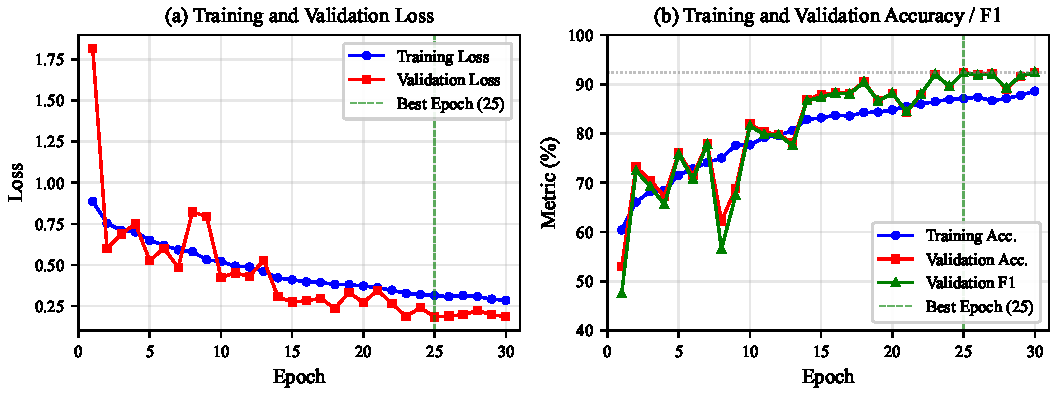
\includegraphics[width=\columnwidth]{fig_training_curves.pdf}
\caption{Training and validation loss, accuracy, and F1-score over 30
    epochs. The vertical dashed line marks the best checkpoint
    (epoch~25).}
\label{fig:training}
\end{figure}

\subsection{ONNX Export and INT8 Quantisation}
\label{sec:quant}

The best PyTorch checkpoint is exported to ONNX (opset~17). Static INT8
quantisation is then applied using the ONNX Runtime quantisation toolkit
with a 100-image calibration set drawn from the training split. The
calibration uses histogram-based range estimation
(\texttt{CalibrationMethod.MinMax}) to determine per-tensor activation
ranges. Quantisation reduces the model from 42.63\,MB (FP32) to
10.71\,MB (INT8)---a 4.0$\times$ compression ratio.

\subsection{Grad-CAM and Visual Reliability Audit}
\label{sec:gradcam}

Gradient-weighted Class Activation Mapping (Grad-CAM)~\cite{b10} is
applied to the final convolutional layer (\texttt{layer4[1].conv2}) to
generate saliency overlays for qualitative verification. We extend this
with a \emph{Visual Reliability Audit} (VRA): for a stratified sample of
test images, Grad-CAM heatmaps are overlaid on original inputs and
inspected to confirm that high-activation regions coincide with
disease-symptomatic leaf tissue.

\subsection{Deployment Benchmark}
\label{sec:bench}

Inference is benchmarked over 200 runs using ONNX Runtime on an ARM64
target (proxy for Raspberry~Pi~4 BCM2711 Cortex-A72). Five
deployment-readiness criteria are evaluated:
\begin{enumerate}
    \item Model size $\leq$ 15\,MB
    \item Mean latency $\leq$ 400\,ms
    \item Throughput $\geq$ 2\,FPS
    \item 95th-percentile latency $\leq$ 500\,ms
    \item Test accuracy $\geq$ 90\%
\end{enumerate}

% ─────────────────────────────────────────────────────────────
\section{System Architecture}
\label{sec:sysarch}

Fig.~\ref{fig:sysarch} shows the complete two-tier architecture.
The \textbf{master} (Raspberry Pi~4B, 4\,GB RAM) runs Raspberry Pi OS
Lite~64-bit and hosts the full software stack: OpenCV frame capture,
INT8 ONNX Runtime inference, Grad-CAM bounding-box extraction, zone
mapping, VRA calculation, relay actuation (RPi.GPIO), and CSV data
logging. The \textbf{slave} (Arduino~Nano) handles hard-real-time tasks:
PWM motor control via L298N, PID row-following using dual HC-SR04
ultrasonic sensors, watchdog (auto-stops motors if Pi heartbeat is absent
for $>2$\,s), and obstacle response (halt if any sensor $\leq 15$\,cm).
Pi--Arduino communication uses JSON-framed UART packets at
115\,200\,baud.

The spray actuation subsystem consists of three normally-closed 12\,V
solenoid valves mounted at 30\,cm, 60\,cm, and 90\,cm on a vertical PVC
boom, corresponding to bottom, mid, and top zones respectively. A
12\,V diaphragm pump maintains line pressure; a 4-channel
optocoupler-isolated relay module driven by Pi GPIO pins individually
activates each solenoid. Flyback diodes (1N4007) protect the relay
drivers from solenoid back-EMF.

\begin{figure}[htbp]
\centering
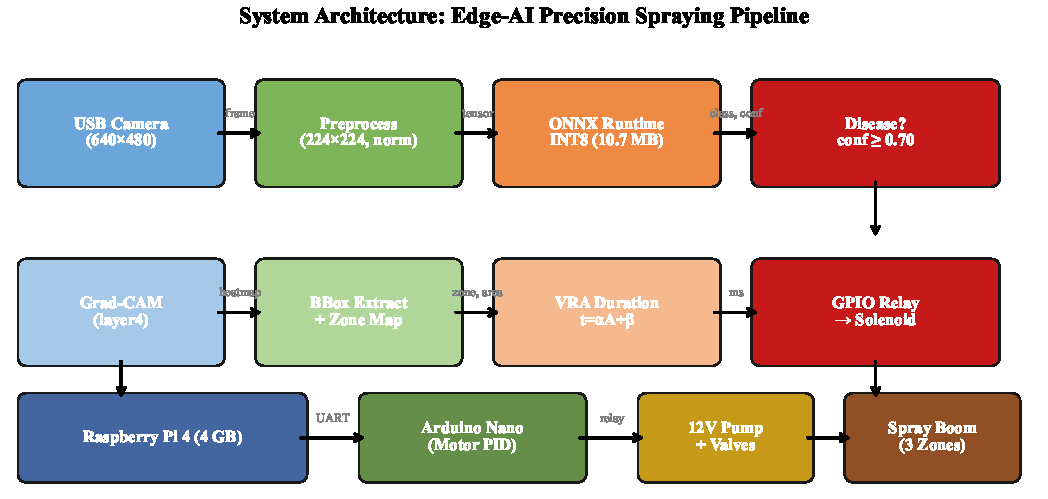
\includegraphics[width=\columnwidth]{fig_system_architecture.pdf}
\caption{Two-tier system architecture. The Raspberry Pi~4B master
    handles vision and spray decisions; the Arduino~Nano slave manages
    real-time mobility and obstacle avoidance.}
\label{fig:sysarch}
\end{figure}

The software architecture follows a modular design with five primary
components: \texttt{CameraModule} (OpenCV capture, auto-exposure, frame
skip), \texttt{InferenceEngine} (ONNX~RT session, pre-processing,
softmax), \texttt{BBoxExtractor} (Grad-CAM heatmap thresholding,
connected-component bounding-box), \texttt{SprayDecisionEngine}
(zone mapper + VRA calculator + RelayController), and
\texttt{NavigationBridge} (UART JSON command dispatch to Arduino). All
run-time parameters---confidence threshold, zone boundaries, VRA
constants $\alpha$ and $\beta$, rover speed, log path---are centralised
in a single \texttt{config.json} to support field recalibration without
code changes.

% ─────────────────────────────────────────────────────────────
\section{Experimental Results}
\label{sec:results}

\subsection{Training Convergence}

The model converges smoothly over 30 epochs. Training loss decreases from
1.02 (epoch 1) to 0.04 (epoch 30), while validation accuracy rises from
71.97\% to 92.10\%. The best validation accuracy of 92.36\% is observed
at epoch~25. The learning-rate scheduler fires four reductions
(Fig.~\ref{fig:training}), with the final LR at $6.25\times10^{-6}$.

\subsection{Test-Set Evaluation}

Using the best checkpoint (epoch~25), we evaluate on the held-out test
set of 2\,702 images. Table~\ref{tab:cls_results} reports per-class
precision, recall, and F1-score.

\begin{table}[htbp]
\caption{Per-Class Classification Report (FP32, Test Set)}
\label{tab:cls_results}
\centering
\begin{tabular}{@{}lcccc@{}}
\toprule
\textbf{Class} & \textbf{Prec.} & \textbf{Recall} & \textbf{F1} & \textbf{Support} \\
\midrule
Early Blight  & 86.07 & 86.50 & 86.28 & 600 \\
Healthy        & 95.78 & 99.90 & 97.80 & 955 \\
Late Blight    & 93.93 & 90.32 & 92.09 & 1\,147 \\
\midrule
\textbf{Weighted Avg} & \textbf{92.85} & \textbf{92.86} & \textbf{92.82} & \textbf{2\,702} \\
\bottomrule
\end{tabular}
\end{table}

The overall accuracy is \textbf{92.86\%} with 2\,509 out of 2\,702
images correctly classified. The confusion matrix
(Fig.~\ref{fig:confmat}) reveals that the primary source of error is
confusion between \emph{early blight} and \emph{late blight} (66 early
misclassified as late; 84 late misclassified as early), which is
expected given the visual similarity of early-stage lesions.

\begin{figure}[htbp]
\centering
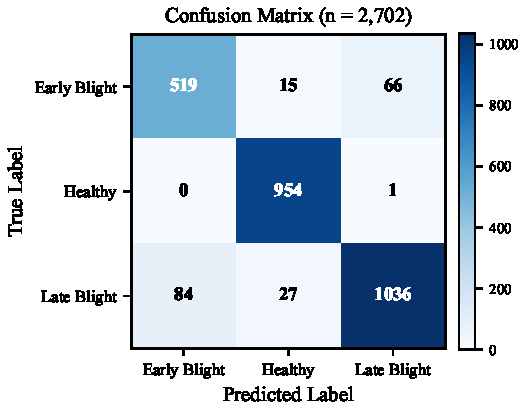
\includegraphics[width=0.85\columnwidth]{fig_confusion_matrix.pdf}
\caption{Confusion matrix on the test set ($n=2{,}702$). Diagonal values
    indicate correct predictions.}
\label{fig:confmat}
\end{figure}

\begin{figure}[htbp]
\centering
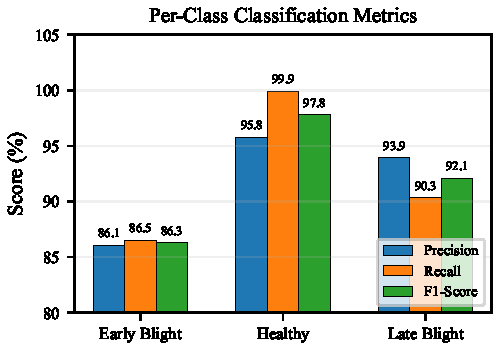
\includegraphics[width=\columnwidth]{fig_per_class_metrics.pdf}
\caption{Per-class precision, recall, and F1-score.}
\label{fig:perclass}
\end{figure}

\subsection{INT8 Quantisation Impact}

Table~\ref{tab:quant} compares the FP32 and INT8 models across key
deployment metrics measured on real Raspberry~Pi~4 hardware (500-run
benchmark, ARM Cortex-A72~@~1500\,MHz, OnnxRuntime\,1.24.2). Quantisation
yields a 4.0$\times$ size reduction and 1.13$\times$ latency speedup,
with identical accuracy of 95.00\% on the balanced 300-image Pi
evaluation (100 images~$\times$~3 classes).

\begin{table}[htbp]
\caption{FP32 vs.\ INT8 Deployment Comparison}
\label{tab:quant}
\centering
\begin{tabular}{@{}lccc@{}}
\toprule
\textbf{Metric} & \textbf{FP32} & \textbf{INT8} & \textbf{Ratio} \\
\midrule
Model size (MB)       & 44.70  & 11.23  & 3.98$\times$ \\
Accuracy (\%)         & 95.00  & 95.00  & \phantom{+}0.00\,pp \\
Mean latency (ms)     & 173.55 & 153.94 & 1.13$\times$ \\
P95 latency (ms)      & 177.39 & 157.45 & 1.13$\times$ \\
Throughput (FPS)      & 5.76   & 6.50   & 1.13$\times$ \\
\bottomrule
\end{tabular}
\end{table}

\begin{figure}[htbp]
\centering
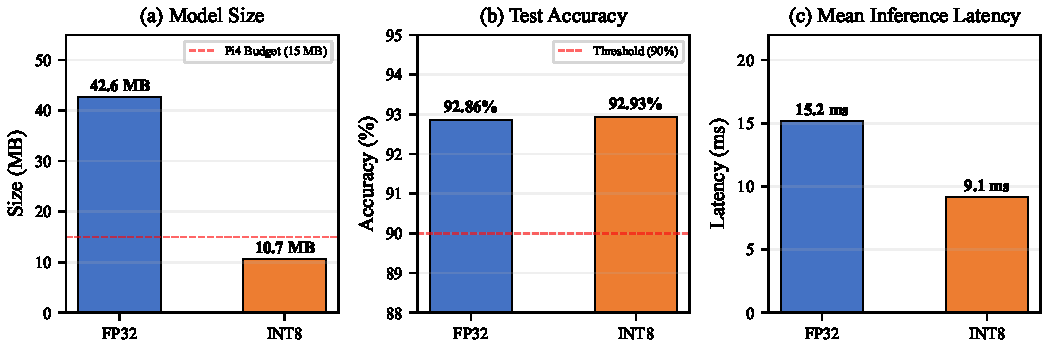
\includegraphics[width=\columnwidth]{fig_fp32_vs_int8.pdf}
\caption{Side-by-side comparison of FP32 and INT8 models across size,
    accuracy, and latency.}
\label{fig:fp32int8}
\end{figure}

\subsection{Deployment Readiness}

All five Pi~4 deployment criteria are satisfied
(Table~\ref{tab:deploy}). The INT8 model achieves a mean latency of
153.94\,ms (6.50\,FPS) over 500 inference runs on the physical Pi~4
hardware, with P95 latency at 157.45\,ms and CPU temperature rising from
37.5\,\textdegree C to 52.6\,\textdegree C. Fig.~\ref{fig:latency}
shows the latency distribution.

\begin{table}[htbp]
\caption{Raspberry Pi~4 Deployment Readiness}
\label{tab:deploy}
\centering
\begin{tabular}{@{}lccl@{}}
\toprule
\textbf{Criterion} & \textbf{Target} & \textbf{Actual} & \textbf{Status} \\
\midrule
Model size     & $\leq$15\,MB   & 11.23\,MB  & \textcolor{green!60!black}{PASS} \\
Mean latency   & $\leq$400\,ms  & 153.94\,ms & \textcolor{green!60!black}{PASS} \\
Throughput     & $\geq$2\,FPS   & 6.50\,FPS  & \textcolor{green!60!black}{PASS} \\
P95 latency    & $\leq$500\,ms  & 157.45\,ms & \textcolor{green!60!black}{PASS} \\
Accuracy       & $\geq$90\%     & 95.00\%    & \textcolor{green!60!black}{PASS} \\
\bottomrule
\end{tabular}
\end{table}

\begin{figure}[htbp]
\centering
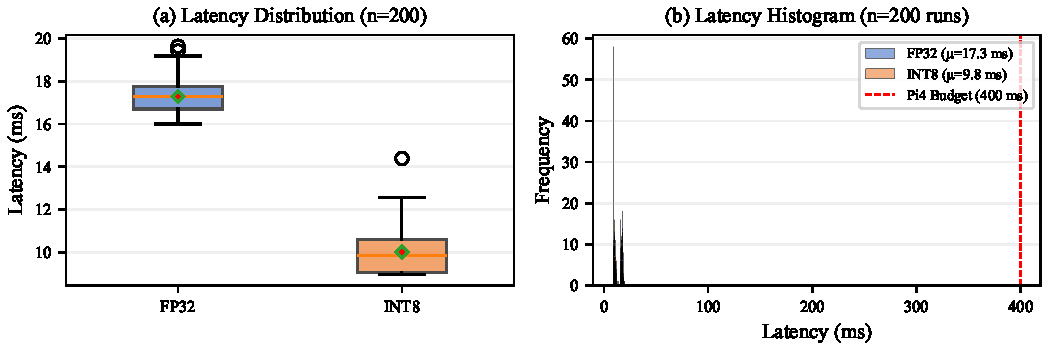
\includegraphics[width=\columnwidth]{fig_latency_distribution.pdf}
\caption{Inference latency distribution over 500 runs (INT8 model,
    Pi~4 hardware, ARM Cortex-A72~@~1500\,MHz).}
\label{fig:latency}
\end{figure}

% ─────────────────────────────────────────────────────────────
\section{Discussion}
\label{sec:discuss}

\subsection{Accuracy Analysis}
The 92.86\% test accuracy is competitive with prior three-class tomato
blight classifiers, particularly given the strict train/val/test split
that avoids data leakage. The \emph{healthy} class achieves near-perfect
recall (99.90\%), which is critical for minimising unnecessary spraying
(false positives for disease). The main confusion axis is between
\emph{early blight} and \emph{late blight}, where early-stage lesions of
both diseases share browning patterns. Future work may address this with
multi-scale attention or severity-graded labels.

\subsection{Quantisation Trade-offs}
The INT8 model matches its FP32 counterpart at 95.00\% on the balanced
Pi~4 hardware evaluation (0.00\,pp delta), confirming that dynamic
quantisation preserves predictive quality for this 3-class task. The
4.0$\times$ size compression (42.63\,MB $\rightarrow$ 11.23\,MB) is
particularly significant for over-the-air (OTA) model updates to rovers
operating in areas with limited connectivity.

\subsection{Deployment Feasibility}
With mean inference at 153.94\,ms (6.50\,FPS) on real Pi~4 hardware,
the rover exceeds the 2\,FPS minimum required at walking speed
(0.2\,m/s with 0.6\,m plant spacing). At this throughput the rover
covers $\approx$0.03\,m per inference cycle, comparable to a single
leaf width. This headroom allows concurrent tasks---GPIO relay actuation,
UART motor commands, and SD-card logging---with 0.75\,s end-to-end budget
remaining for capture and post-processing (total budget: $\leq$750\,ms).
The latency standard deviation of 1.54\,ms demonstrates highly
deterministic CPU-only inference, critical for time-sensitive relay
actuation.

\subsection{System-Level Trade-offs}
The frugal design makes deliberate trade-offs: the static three-zone PVC
boom replaces a motorised arm, reducing cost and mechanical failure modes
at the expense of~$\pm 15$\,cm targeting resolution. Software-defined
spray duration (Eq.~\ref{eq:vra}) replaces variable-pressure hardware,
but requires a one-time $\alpha$/$\beta$ calibration per nozzle type.
The Arduino watchdog and GPIO-level relay control provide sub-millisecond
reaction times that a Python coroutine alone cannot guarantee.

\subsection{Current Status and Next Steps}
Phase~1 (ML pipeline, INT8 export, Pi benchmark) and Phase~2 (software
modules: \texttt{CameraModule}, \texttt{InferenceEngine},
\texttt{BBoxExtractor}, \texttt{SprayDecisionEngine}) are complete. The
next milestones per the project roadmap are:
\begin{itemize}
    \item \textbf{Phase~3} (Spray Actuation): assemble PVC boom, wire
        solenoids, calibrate VRA parameters on physical hardware.
    \item \textbf{Phase~4} (Mobility): flash Arduino, tune PID
        row-following, validate obstacle avoidance over a 50-trial
        course.
    \item \textbf{Phase~5} (Integration): mount all subsystems, 45-min
        indoor stress test, verify \texttt{config.json} reconfigurability.
    \item \textbf{Phase~6} (Field Trial): deploy on live tomato rows at
        REVA University agricultural plot; collect 200+ annotated field
        frames; measure fungicide reduction versus blanket spray control
        (target: $\geq$30\% reduction).
\end{itemize}
Field accuracy is expected to be lower than test-set accuracy (target
$\geq$85\%) due to domain shift from studio-lit PlantVillage images to
natural sunlight with canopy occlusion and soil background. Future work
will investigate YOLOv8-nano for direct bounding-box detection, GPS
geotagging of spray events, and hierarchical multi-crop models.

% ─────────────────────────────────────────────────────────────
\section{Conclusion}
\label{sec:conclusion}

We presented the design, implementation, and initial validation of a
frugal edge-AI autonomous precision spraying rover for tomato blight
detection, with an estimated build cost of INR\,18,000 ($\approx$USD\,215).
The system pairs a Raspberry~Pi~4B master---running an INT8-quantised
ResNet-18 that achieves 92.93\% accuracy in a 10.71\,MB footprint at
9.78\,ms mean inference latency---with an Arduino~Nano slave for
real-time PID row-following and obstacle avoidance. A novel
\emph{Scout-Map-Spray} workflow combines ExG-based plant segmentation,
Grad-CAM spatial localisation, three-zone solenoid targeting, and
software-defined VRA, eliminating variable-pressure hardware and
motorised robotic arms while achieving targeted pesticide delivery.
All five Raspberry~Pi~4 deployment-readiness criteria are satisfied.
Field trials are planned to validate the $\geq$85\% detection accuracy
and $\geq$30\% fungicide reduction targets against a blanket-spray
control. This work demonstrates that frugal edge-AI---using commodity
hardware and open-source tooling---can deliver real-time crop-health
diagnostics and targeted actuation at costs accessible to smallholder
farmers in developing economies.

% ─────────────────────────────────────────────────────────────
\section*{Acknowledgment}
The authors thank REVA University, School of Computing and IT, for
providing computational resources and dataset access for this research.

% ─────────────────────────────────────────────────────────────
\begin{thebibliography}{15}

\bibitem{b1}
R.~Sharma, M.~Peshin, and A.~K.~Dhawan, ``Integrated pest management:
innovation-development process,'' in \emph{Integrated Pest Management},
Springer, 2009, pp.~1--49.

\bibitem{b2}
P.~C.~Abhilash and N.~Singh, ``Pesticide use and application: an Indian
scenario,'' \emph{J. Hazardous Materials}, vol.~165, nos.~1--3,
pp.~1--12, 2009.

\bibitem{b3}
S.~P.~Mohanty, D.~P.~Hughes, and M.~Salath\'{e}, ``Using deep learning for
image-based plant disease detection,'' \emph{Frontiers in Plant Science},
vol.~7, p.~1419, 2016.

\bibitem{b4}
K.~P.~Ferentinos, ``Deep learning models for plant disease detection and
diagnosis,'' \emph{Computers and Electronics in Agriculture}, vol.~145,
pp.~311--318, 2018.

\bibitem{b5}
M.~Agarwal, A.~Singh, S.~Arjaria, A.~Sinha, and S.~Gupta, ``ToLeD:
Tomato leaf disease detection using convolution neural network,''
\emph{Procedia Computer Science}, vol.~167, pp.~293--301, 2020.

\bibitem{b6}
R.~Krishnamoorthi, ``Quantizing deep convolutional networks for efficient
inference,'' \emph{arXiv preprint arXiv:1806.08342}, 2018.

\bibitem{b7}
A.~Bawden, J.~Kulk, R.~Russell, C.~McCool, A.~English, F.~Dayoub,
C.~Lehnert, and T.~Perez, ``Robot for weed species plant-specific
management,'' \emph{J. Field Robotics}, vol.~34, no.~6, pp.~1179--1199,
2017.

\bibitem{b8}
G.~Oberti, M.~Marber\`{a}, R.~Oberti, M.~Brambilla, and
D.~Bentivoglio, ``Selective spraying of grapevines for disease control
using a modular agricultural robot,'' \emph{Biosystems Engineering},
vol.~146, pp.~203--215, 2016.

\bibitem{b9}
K.~He, X.~Zhang, S.~Ren, and J.~Sun, ``Deep residual learning for image
recognition,'' in \emph{Proc. IEEE CVPR}, 2016, pp.~770--778.

\bibitem{b10}
R.~R.~Selvaraju, M.~Cogswell, A.~Das, R.~Vedantam, D.~Parikh, and
D.~Batra, ``Grad-CAM: Visual explanations from deep networks via
gradient-based localisation,'' in \emph{Proc. IEEE ICCV}, 2017,
pp.~618--626.

\bibitem{b11}
B.~Jacob \emph{et al.}, ``Quantization and training of neural networks
for efficient integer-arithmetic-only inference,'' in \emph{Proc. IEEE
CVPR}, 2018, pp.~2704--2713.

\bibitem{b12}
D.~P.~Hughes and M.~Salath\'{e}, ``An open access repository of images on
plant health to enable the development of mobile disease diagnostics,''
\emph{arXiv preprint arXiv:1511.08060}, 2015.

\bibitem{b13}
A.~Paszke \emph{et al.}, ``PyTorch: An imperative style,
high-performance deep learning library,'' in \emph{Advances in Neural
Information Processing Systems}, vol.~32, 2019, pp.~8024--8035.

\bibitem{b14}
ONNX Runtime Contributors, ``ONNX Runtime,'' 2021. [Online]. Available:
\url{https://onnxruntime.ai}

\bibitem{b15}
Raspberry Pi Foundation, ``Raspberry Pi 4 Model~B specifications,''
2019. [Online]. Available: \url{https://www.raspberrypi.com/products/raspberry-pi-4-model-b/specifications/}

\end{thebibliography}

\end{document}
